\documentclass[conference]{IEEEtran}
\IEEEoverridecommandlockouts
% The preceding line is only needed to identify funding in the first footnote. If that is unneeded, please comment it out.
\usepackage{cite}
%\usepackage[brazil]{babel} % pacote portugues 
\usepackage[utf8]{inputenc} % pacote para acentuacao direta
\usepackage{amsmath,amssymb,amsfonts}
\usepackage{algorithmic}
\usepackage{graphicx}
\usepackage{textcomp}
\usepackage{xcolor}
\usepackage{subcaption}
\def\BibTeX{{\rm B\kern-.05em{\sc i\kern-.025em b}\kern-.08em
    T\kern-.1667em\lower.7ex\hbox{E}\kern-.125emX}}
\begin{document}

\title{SNB - Evolutionalary Computing in Smart Grid
%*\\{\footnotesize \textsuperscript{*}Note: Sub-titles are not captured in Xplore and should not be used}
}

\author{\IEEEauthorblockN{1º Daniel Alexandre Oleinik}
\IEEEauthorblockA{\textit{CPGEI - COORD.PROG.POS-GRAD.INFOR.IND.ENG.ELET} \\
\textit{UTFPR - Universidade Tecnológica Federal do Paraná}\\
Curitiba, Brasil}
\and
\IEEEauthorblockN{2º Mauro Sergio Pereira Fonseca}
\IEEEauthorblockA{\textit{CPGEI - COORD.PROG.POS-GRAD.INFOR.IND.ENG.ELET} \\
\textit{UTFPR - Universidade Tecnológica Federal do Paraná}\\
Curitiba, Brasil}
\and
\IEEEauthorblockN{3º Anelise Munaretto}
\IEEEauthorblockA{\textit{CPGEI - COORD.PROG.POS-GRAD.INFOR.IND.ENG.ELET} \\
\textit{UTFPR - Universidade Tecnológica Federal do Paraná}\\
Curitiba, Brasil}
}

\maketitle

\begin{abstract}
The growth  of energy consumption from non-renewable and finite sources is encouraging the advance in the development of new power generation options. These options, when included to the current electric power generation system should demand new requirements from the communication system used with the power distribution network equipment, motivating the development of the real Smart Grid. This document proposes a method for enhancement and optimization of a network grid, built in optic fiber and using mesh topology by changing the physical layer of the network together with smart reactive management.
\end{abstract}

\begin{IEEEkeywords}
Smart Grid, Optical switch, IP network, Mesh Network, Optimization, Latency, Genetic Algorithms, Evolutional Computing
\end{IEEEkeywords}

\section{Introduction}
The utilization of fossil fuels, global warming, and the global population boom have become more and more important topics. They are speeding up the development of renewable sources of energy like wind and solar energy generation since these new sources promise to have a lower impact on the global environment. The integration of these power sources in the current energy distribution and transmission system demands the existence of a new communication system that can offer a faster, more efficient and trustable infra-structure \cite{Art-Gungor2013}.

Still according to \cite{Art-Gungor2013}, the renewable sources of energy have the natural tendency of non-centralized installation, like the solar or wind power generation, since they are geographic or climatic dependent. Therefore, these technologies usages should change the current energy distribution system to a big distributed energy generation system, making it necessary to use an infrastructure capable of meeting the communication needs of the big variety of sensors, actuators, and elements used in the control of the new energy generation and distribution. Which in short means the concept of Smart Grid.

This document presents the simulation results of using optical switches in strategic network points (considering an optical network infrastructure) to bypass specific equipment with no impact in any communication, resulting in a layer 1 optimization focusing in latency values.

\section{Proposal}

\subsection{Basic Concepts}

\subsubsection{Mesh Network Topology}
There are many different ways to interconnect hosts. According to \cite{Book-Kurose2013} a computer network is nothing else than a communication infrastructure that offers services to distributed applications using links with ``packet switches’’. The network topology depends on the interconnection, and the most common topologies are bus, ring, star, tree, and mesh.

The mesh topology is characterized by the creation of a big, or sometimes full, connection between the hosts, producing many redundant paths between messages origin and destination. It grants a high disponibility and availability to this type of network since even in an infrastructure or equipment failure the communication is not compromised. The Figure \ref{fig_topologia_multiplo_mesh} shows a basic mesh network. It is possible to see that in this topology there are costs related to packet routing, forwarding and process because, unless the origin and destination of the packet are directly connected, it is necessary to repeat the packets in the intermediary points to establish the communication.

\begin{figure}[htbp]
	\centering
	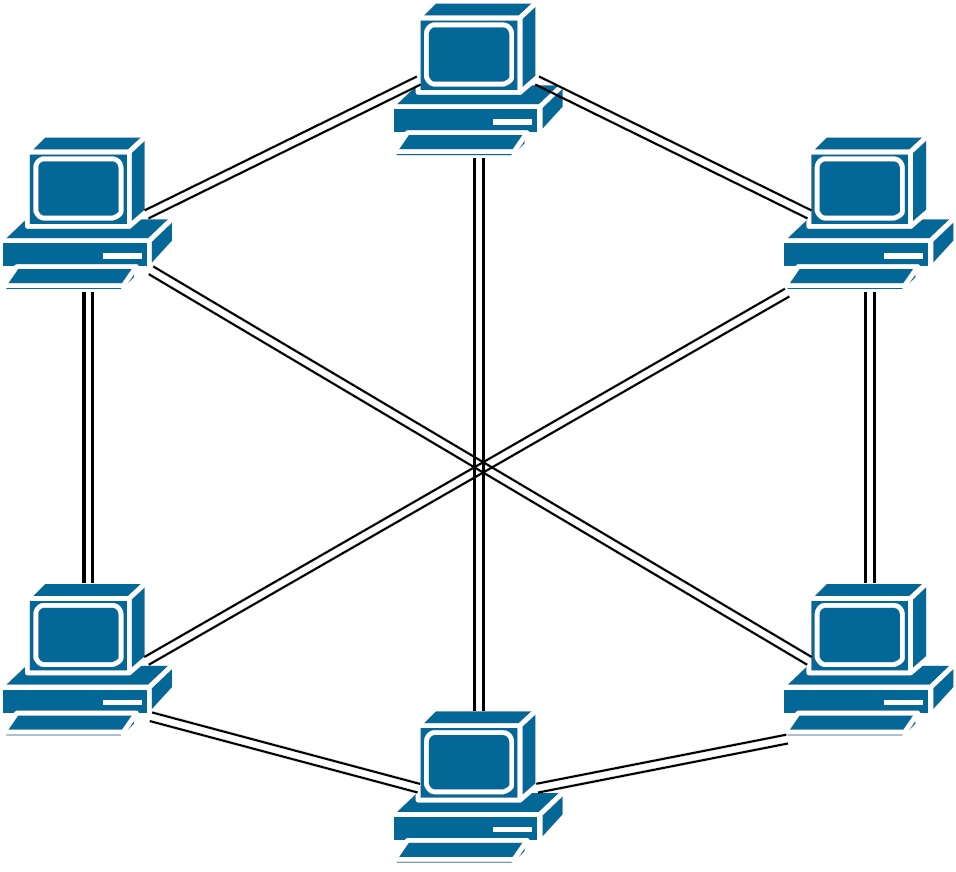
\includegraphics[width=0.15\textwidth]{./figuras/Topologia-Mesh.jpg} % <- formatos PNG, JPG e PDF
	\caption{Basic mesh topology.}
	\label{fig_topologia_multiplo_mesh}
\end{figure}

\subsubsection{Optical Switch}
The communication inside optical networks is done by light signals with different frequencies (usually called signal colors). It implies in different wavelengths, and big networks with many colors or $\lambda$, like current optical networks, have some central types of equipment called OXCs or Optical Cross Connect

The OXCs can realize the internal signal routing in a pure optic, pure electric ou hybrid way \cite{Book-Ramaswami2010}, and in this last case, they are called translucid OXCs. This kind of equipment is largely used in the current optical networks and they are also known as OEO or Optical-Electrical-Optical.

Optical switches, on the other hand, are special optic components that can divert the light using a reflective prism. Figure \ref{fig_chaveador_optico} shows the simplified internal diagram of an optical switch, it is possible to notice that its operation is analog to an electric relay.

\begin{figure}[htbp]
	\centering
	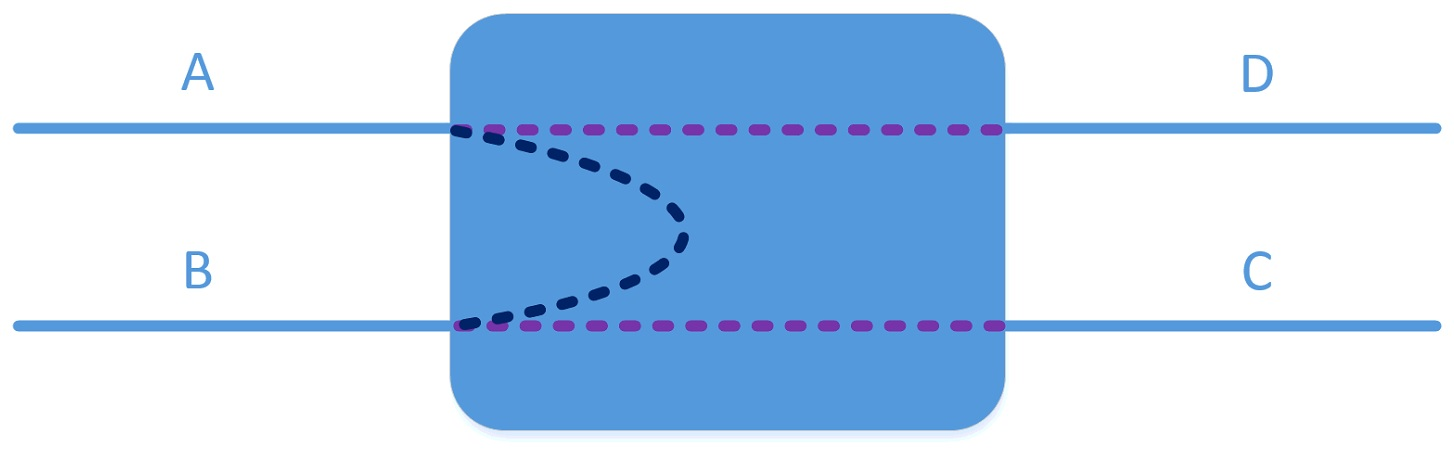
\includegraphics[width=0.3\textwidth]{./figuras/Switch_optico.jpg} % <- formatos PNG, JPG e PDF
	\caption[Exemplo básico chaveador óptico]{Simplified internal diagram of an optical switch. In one state the light is forwarded from A to D and from B to C, when activated the light is transmitted from A to B. Adapted from \cite{Accelink2014}}
	\label{fig_chaveador_optico}
\end{figure}

It is important to say that an optical switch is essentially a passive component. When the internal reflective prism is activated the light is transmitted to the related output with no changes, in other words, this component deviates the light signal. However, the usage of an optical switch in an OEO equipment can give it the capacity to deviate optic signals when it is necessary, transforming it in a translucid OXC. 

\subsubsection{Delays in optical networks}
The delays caused by electrical equipment used in optical fibers networks have many sources such as processing power and media conversions. To every equipment in an optical network, it is possible to consider at least two media conversions (optic-electric-optic).

Thus, every time a packet travels in an optic network it suffers delays, that can be translated to latency, in every node of the circuit. These delays must be added in order to determine the total link latency. Figure \ref{fig_latency_link} shows the latency accumulation in an optical link between two points. 

\begin{figure} [htbp]% normalmente utilizar [!t]
	\centering
	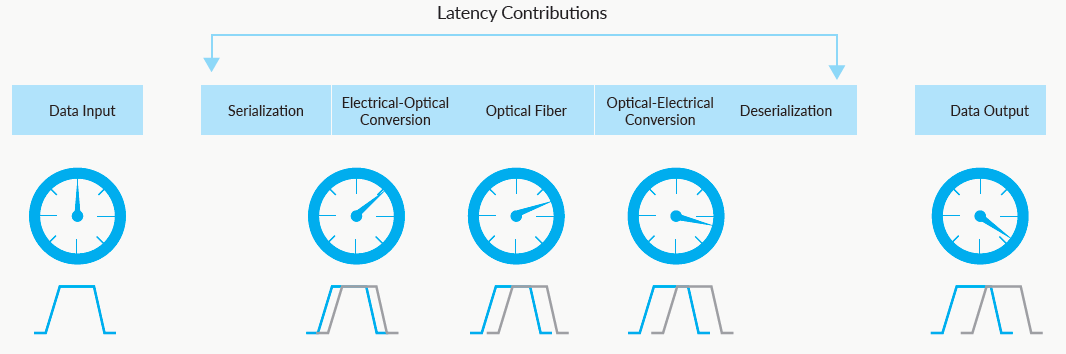
\includegraphics[width=0.4\textwidth]{./figuras/latency-link.png}
	\caption{Communication latency between two points using an optical link. The main latency insertion points are a result of the conversion electric-optic, transmission, conversion optic-electric, process, and deserialization. Source \cite{Art-Coffe2017}}
	\label{fig_latency_link}
\end{figure}

\subsubsection{Energy Distribution Smart Grids}
The Smart Grid offers a big variety of services that were not offered before (considering the conventional energy distribution networks). In \cite{Art-Ma2013} there is a small report about some of the benefits of the smart grids as the better energy management, remote operation monitoring, assertiveness in fail recovery, lower waste due to the better control of production and demand, lower number of field teams and others. Table \ref{tab_comparacao_grids} compares the main differences between current energy distribution networks and Smart Grids.

\begin{table}[tbp]
\begin{tabular}{l|l|l|}
\cline{2-3}
 & \multicolumn{1}{c|}{\textbf{Existing Grid}} & \multicolumn{1}{c|}{\textbf{Smart Grid}} \\ \hline
\multicolumn{1}{|l|}{\textbf{Information Flow}} & Unidiretional & Bidiretional \\ \hline
\multicolumn{1}{|l|}{\textbf{Electricity generation}} & Centralized generation & Distributed generation \\ \hline
\multicolumn{1}{|l|}{\textbf{Grid Topology}} & Radial & Network \\ \hline
\multicolumn{1}{|l|}{\textbf{Sensors}} & Few sensors & Lots of sensors \\ \hline
\multicolumn{1}{|l|}{\textbf{Monitoring ability}} & Usually blind & Self-monitoring \\ \hline
\multicolumn{1}{|l|}{\textbf{Outage recovery}} & Manual restoration & Self-reconfiguration \\ \hline
\multicolumn{1}{|l|}{\textbf{Testing}} & Manual check & Remote check \\ \hline
\multicolumn{1}{|l|}{\textbf{Control ability}} & Limited control & Pervasive control \\ \hline
\multicolumn{1}{|l|}{\textbf{Control type}} & Passive control & Active control \\ \hline
\multicolumn{1}{|l|}{\textbf{Overall efficiency}} & Low & High \\ \hline
\multicolumn{1}{|l|}{\textbf{Environmental pollution}} & High & Low \\ \hline
\end{tabular}
\caption{comparison between basic parameters of normal and smart grid. Source: adapted from \cite{Art-Ma2013}}
\label{tab_comparacao_grids}
\end{table}
	
\subsection{SNB - Selective Network Bypass}
The SNB was specifically developed to optimize latency in optical networks by using optical switches in strategic points of the network. In other words, the SBN manipulates the physical layer of the network, consequently changing its topology. Thus, equipment in specific positions of the network can be deviated without any necessity of media conversion or even processing, resulting in the minimal latency insertion possible.

The SNB operates completely independent of the routing protocol used in the network changing only its topology, because of that it can be used even with layer two protocols. The network points of optical switch activation can be chosen in graph branches with many nodes (hops) or they can be planned to establish specific communication routes to the critical points of the system, enabling a Service Level Agreement over the physical layer. By using SNB it is possible to reduce the networks graph and create a new set of connections not present in the original network and also a new variety of possible paths between nodes.

Every time the SNB activate a bypass the two related edges are unified avoiding their vertex, creating a new graph with a distance between two final vertexes with one less vertex, as represented in Figure \ref{fig-bypass-exemplo}.

\begin{figure}[htbp]
	\centering
	\begin{subfigure}[t]{0.2\textwidth}
		\centering
		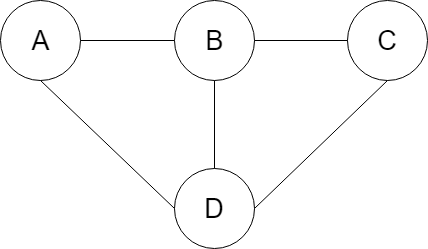
\includegraphics[width=0.9\textwidth]{./figuras/Bypass-exemplo-A.png} % <- formatos PNG, JPG e PDF
		\caption{Chaveador óptico desativado}
		\label{fig_bypass_exemplo_A}
	\end{subfigure}%
	~
	\begin{subfigure}[t]{0.2\textwidth}
		\centering
		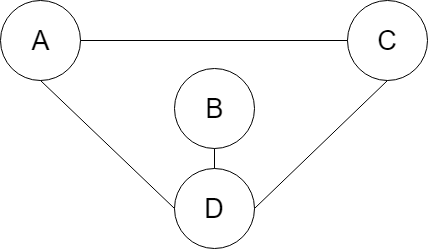
\includegraphics[width=0.9\textwidth]{./figuras/Bypass-exemplo-B.png} % <- formatos PNG, JPG e PDF
	\caption{Chaveador óptico ativado}
	\label{fig_bypass_exemplo_B}
	\end{subfigure}
	\caption{Optical switch activation effect. In \ref{fig_bypass_exemplo_A} it is possible to see the original network with 2 hops between vertexes A and C. Em \ref{fig_bypass_exemplo_B} after activation of the component in vertex B, there is only 1 hop between the vertexes A and C. 	}
	\label{fig-bypass-exemplo}
\end{figure}

\subsubsection{Operation}
The network of Figure \ref{BSN-example-network} was generated to evaluate the operation of SNB. This network is represented by a simple graph with valency 3 and mesh topology. This graph was submitted to STP protocol to calculate the optimal paths to every vertex from the origin vertex (arbitrarily chosen as 1). The result is shown in Figure \ref{BSN-example-network-tree}, which actually represents the minimal spanning tree for the graph from Figure \ref{BSN-example-network}.

The same graph from Figure \ref{BSN-example-network} was submitted to the SNB execution. As a result, it was decided to activate the optical switch in vertex 7, linking the vertex 1 directly to 4 and generating the graph of Figure \ref{BSN-example-opt-switch}. This graph, when submitted to the calculation of the optimal paths, also using STP protocol, results in Figure \ref{BSN-example-rede-otimizada}, where it is possible to see a decrease in depth compared with the shown in Figure \ref{BSN-example-network-tree}.

\begin{figure}[t!]
	\centering
	\begin{subfigure}[t]{0.2\textwidth}
		\centering
		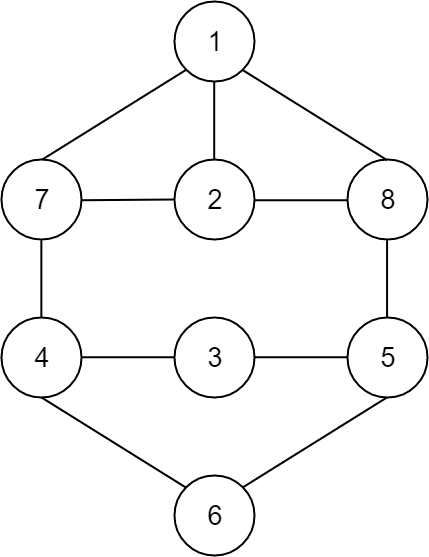
\includegraphics[width=0.7\textwidth]{./figuras/BSN-ex-network-generation.png} % <- formatos PNG, JPG e PDF
		\caption{Generated network}
		\label{BSN-example-network}
	\end{subfigure}%
	~
	\begin{subfigure}[t]{0.2\textwidth}
		\centering
		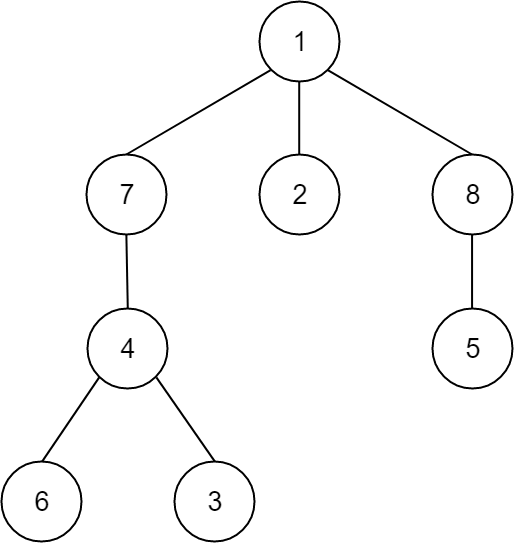
\includegraphics[width=0.7\textwidth]{./figuras/BSN-ex-network-generation-tree.png} % <- formatos PNG, JPG e PDF
	\caption{Network tree}
	\label{BSN-example-network-tree}
	\end{subfigure}
	~
	\begin{subfigure}[t]{0.2\textwidth}
		\centering
		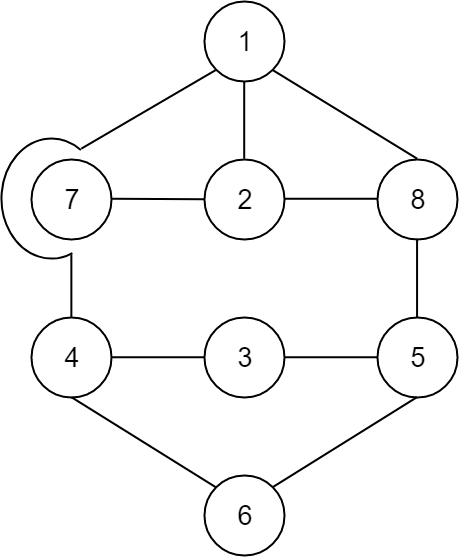
\includegraphics[width=0.7\textwidth]{./figuras/BSN-ex-bypass.png} % <- formatos PNG, JPG e PDF
	\caption{Optical switch activated}
	\label{BSN-example-opt-switch}
	\end{subfigure}
	~
	\begin{subfigure}[t]{0.2\textwidth}
		\centering
		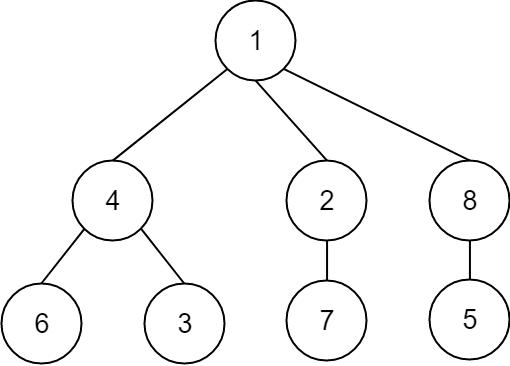
\includegraphics[width=0.7\textwidth]{./figuras/BSN-ex-network-final.png} % <- formatos PNG, JPG e PDF
	\caption{Resulting network}
	\label{BSN-example-rede-otimizada}
	\end{subfigure}
	\caption{SNB operation example. SNB can reduce the depth of a network generating new connection possibilities by changing its the physical layer}
	\label{fig-bsn-exemplo}
\end{figure}

It is possible to notice that the network’s depth, directly related to the communication latency, is reduced impacting in the latency value for the communication between the related nodes. To this example the maximal depth was reduced from 3 to 2 (33,33\%), impacting directly in the latency since there is no more media conversion or even processing in the deviated node, as shown in Figure \ref{fig_latency_link}.

\subsubsection{Total network cost and Individual cost}
The total network cost is defined as the sum of every individual cost (hop number) to the communication in each one of the network links. Thus, using the example network from Figure \ref{BSN-example-network-tree} it is possible to generate the Table \ref{tab-custo-rede-BSN-example-network-tree} that shows the individual costs for the communication from every node to the root node and also the total network cost. On the other hand, using the network represented in Figure \ref{BSN-example-rede-otimizada}, optimized by SNB, the results for individual and total costs are shown in Table \ref{tab-custo-rede-bsn-otimizada}.

\begin{table}[t!]
	\centering
		%\begin{table}[]
			\begin{tabular}{llllll}
			\hline
			\multicolumn{1}{|l|}{\textbf{Destination node}} & \multicolumn{4}{c}{\textbf{Path}} & \multicolumn{1}{c|}{\textbf{Cost}} \\ \hline
			\multicolumn{1}{|l|}{\textbf{2:}} & 1 & 2 &  & \multicolumn{1}{l|}{} & \multicolumn{1}{l|}{1} \\ \hline
			\multicolumn{1}{|l|}{\textbf{3:}} & 1 & 7 & 4 & \multicolumn{1}{l|}{3} & \multicolumn{1}{l|}{3} \\ \hline
			\multicolumn{1}{|l|}{\textbf{4:}} & 1 & 7 & 4 & \multicolumn{1}{l|}{} & \multicolumn{1}{l|}{2} \\ \hline
			\multicolumn{1}{|l|}{\textbf{5:}} & 1 & 8 & 5 & \multicolumn{1}{l|}{} & \multicolumn{1}{l|}{2} \\ \hline
			\multicolumn{1}{|l|}{\textbf{6:}} & 1 & 7 & 4 & \multicolumn{1}{l|}{6} & \multicolumn{1}{l|}{3} \\ \hline
			\multicolumn{1}{|l|}{\textbf{7:}} & 1 & 7 &  & \multicolumn{1}{l|}{} & \multicolumn{1}{l|}{1} \\ \hline
			\multicolumn{1}{|l|}{\textbf{8:}} & 1 & 8 &  & \multicolumn{1}{l|}{} & \multicolumn{1}{l|}{1} \\ \hline
			 & \multicolumn{4}{l}{\textbf{Total Cost}} & \textbf{13}
			\end{tabular}
		\caption{Calculo de custo - Rede Figura \ref{BSN-example-network-tree}}
		\label{tab-custo-rede-BSN-example-network-tree}
		%\end{table}
\end{table}
		
\begin{table}[t!]
	\centering
			%\begin{table}[]
			\begin{tabular}{lllll}
			\hline
			\multicolumn{1}{|l|}{\textbf{Destination node}} & \multicolumn{3}{c}{\textbf{Path}} & \multicolumn{1}{c|}{\textbf{Cost}} \\ \hline
			\multicolumn{1}{|l|}{\textbf{2:}} & 1 & 2 & \multicolumn{1}{l|}{} & \multicolumn{1}{l|}{1} \\ \hline
			\multicolumn{1}{|l|}{\textbf{3:}} & 1 & 4 & \multicolumn{1}{l|}{3} & \multicolumn{1}{l|}{2} \\ \hline
			\multicolumn{1}{|l|}{\textbf{4:}} & 1 & 4 & \multicolumn{1}{l|}{} & \multicolumn{1}{l|}{1} \\ \hline
			\multicolumn{1}{|l|}{\textbf{5:}} & 1 & 8 & \multicolumn{1}{l|}{5} & \multicolumn{1}{l|}{2} \\ \hline
			\multicolumn{1}{|l|}{\textbf{6:}} & 1 & 4 & \multicolumn{1}{l|}{6} & \multicolumn{1}{l|}{2} \\ \hline
			\multicolumn{1}{|l|}{\textbf{7:}} & 1 & 2 & \multicolumn{1}{l|}{7} & \multicolumn{1}{l|}{2} \\ \hline
			\multicolumn{1}{|l|}{\textbf{8:}} & 1 & 8 & \multicolumn{1}{l|}{} & \multicolumn{1}{l|}{1} \\ \hline
			 & \multicolumn{3}{l}{\textbf{Total Cost}} & \textbf{11}
			\end{tabular}
	\caption{Calculo de custo - Rede Figura \ref{BSN-example-rede-otimizada}}
	\label{tab-custo-rede-bsn-otimizada}
	%\end{table}
	\label{tab_calc_custo}
\end{table}

From the data comparison between Tables \ref{tab-custo-rede-BSN-example-network-tree} and \ref{tab_calc_custo} it is clear that the total network cost was optimized approximately 15,4\%, for the cost to destinations 3 and 6 it was possible to reach an improvement of 33,33\% and for destinations 4 and 7 50\% of improvement.

\subsubsection{Implementation}
The SNB algorithm is based on evolutionary computing. The optimization strategy used involves the representation of the network in an array, where every position represents one of the nodes and its value represents the activation of the respective optical switch. Then, this array is considered as a chromosome and used in a Genetic Algorithm with the goal of reducing the fitness function of the problem. This function can be translated as the total cost of the network.

Consequently, to reduce the total network cost, it is necessary to reduce the individual costs and it natural that the longer branches of the network graph (branches with higher costs) are more impacted. In this way, although the main goal is to optimize the latency for all network, it is possible to adequate the fitness function to have more priority in reducing the high latency destinations. 

\subsection{Results}

\subsubsection{Improvements in Total Cost}
To evaluate the performance of SNB were used networks randomly created from 5 to 100 nodes with an increment of 5 units, it means, were generated networks with 5, 10, 15 and so on until 100 nodes. From the results using 300 different networks a total cost improvement graph was generated and it is shown in Figure \ref{fig_graph_bsn_medio_all}. This graph was generated considering a confidence interval of 98\%.

\begin{figure} [ht]% normalmente utilizar [!t]
	\centering
	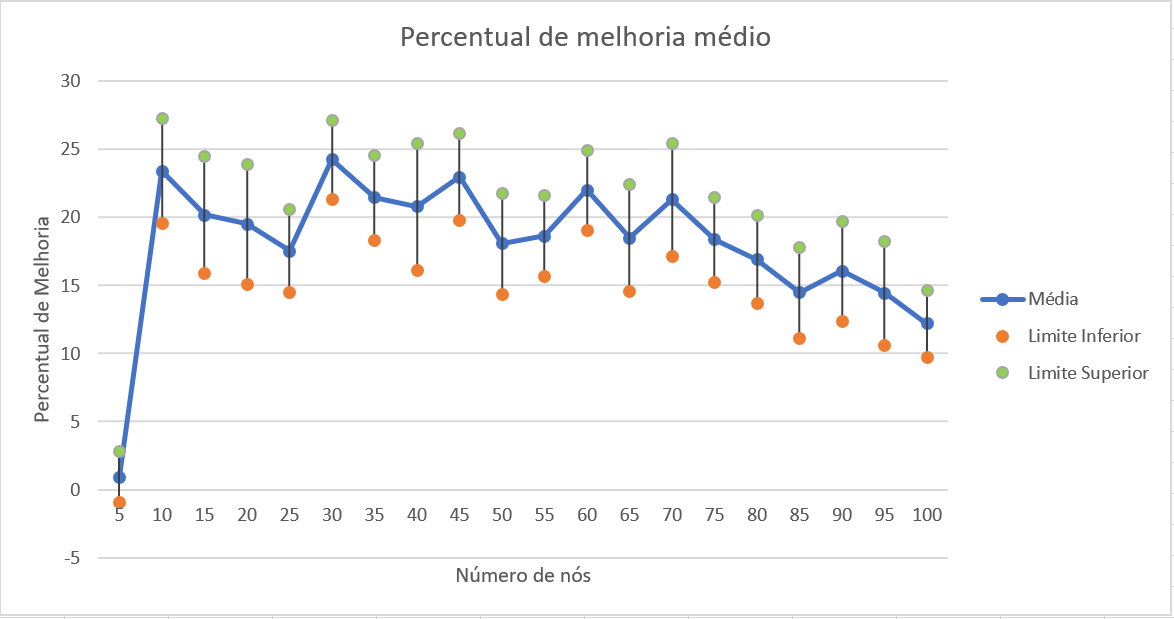
\includegraphics[width=0.49\textwidth]{./figuras/BSN-resultados-medios-all2.png} % <- formatos PNG, JPG e PDF
	\caption{Percentage comparison of average results in total cost improvement considering different size networks and a confidence interval of 98\%.}
	\label{fig_graph_bsn_medio_all}
\end{figure}

\subsubsection{Improvements in Individual Cost}
Analyzing the individual costs from the networks used to generate the graph shown in Figure \ref{fig_graph_bsn_medio_all} it is possible to generate the Figure \ref{fig_graph_melhoria_por_custo}. Here it is possible to clearly notice a significant and increasing improvement in cost for the routes when they grow. It means, when the route is big the optimization is also big. 

Considering a hypothetic network branch with 100 hops in the original topology, based on Figure \ref{fig_graph_melhoria_por_custo} it is possible to predict that after the utilization of SNB this same branch will result in a new path with approximately 73 hops, representing a reduction of 27\% when compared to the original topology. In other words, some points of the city that couldn’t be included in the SG project due to the big distance to the NOC, now can be reached since the latency is significantly reduced, representing a big save to the power electric company

\begin{figure} [ht]% normalmente utilizar [!t]
	\centering
	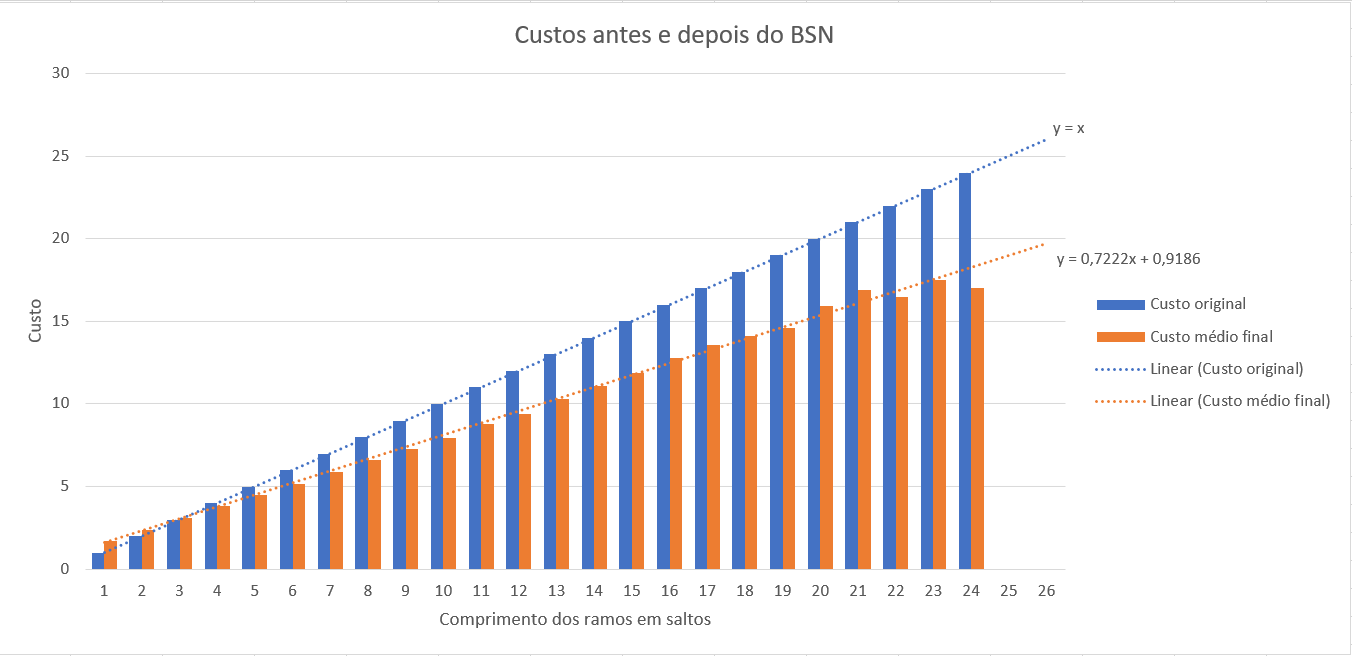
\includegraphics[width=0.49\textwidth]{./figuras/Melhoria-por-custo.png} % <- formatos PNG, JPG e PDF
	\caption{Comparative graph of the average results from improvements in individual costs for each route.}
	\label{fig_graph_melhoria_por_custo}
\end{figure}


\section{Conclusion}
By using the SNB it is possible to notice a sensitive improvement in the cost/depth network parameters to the detriment of the width comparing the original and the resulting network graphs. In other words, the SNB is capable to convert a depth network in a wide network, obviously limited to the connexion already existents in the original network.

Analyzing Figure \ref{fig_graph_bsn_medio_all} it is clear to see an efficiency reduction of the methodology in the decrease of the total cost when it is used in big networks (with many nodes). Considering that the total cost is given by the sum of the all individual costs between all nodes and the root one, it is expected just a few connections with high-cost values, it means, the network should have much more connections with low cost than high cost. Thus the contribution of the optimization of these routes to the total cost is low. Besides that, with many nodes in a mesh network, higher is the number of available routes. It means that in a network with a high level of multipath it is expected that the optimal routes already have a small cost even with no topology changes.

In contrast, the same idea is not applicable considering the individual cost in each branch, which in general represents the biggest worry in this kind of application. According to the presented in Figure \ref{fig_graph_melhoria_por_custo}, in branches with many hops, which represents the real bottleneck in smart grid networks, the improvement is every time bigger after the SNB usage.

As a secondary but very important consequence, the usage of the proposal can permit the inclusion of points originally out of the smart grid network, due to the distance or latency limit, without the necessity of construction of a new NOC. It represents a bigger presence and a big economy to the electric power company. 


\bibliographystyle{IEEEtran}
\bibliography{IEEEabrv,SMMC2018}


\end{document}
